% ============================================================
% DIAGRAM: McCulloch-Pitts Neuron (1943)
% ============================================================
% Caption: Figure 1.1: The McCulloch-Pitts neuron model.
%          (Adapted from McCulloch & Pitts, 1943, p. 117)
% ============================================================

\documentclass[tikz,border=10pt]{standalone}
\usepackage{tikz}
\usepackage{amsmath}
\usepackage{amsfonts}

\usetikzlibrary{shapes,arrows,positioning,fit,calc,backgrounds}

\begin{document}

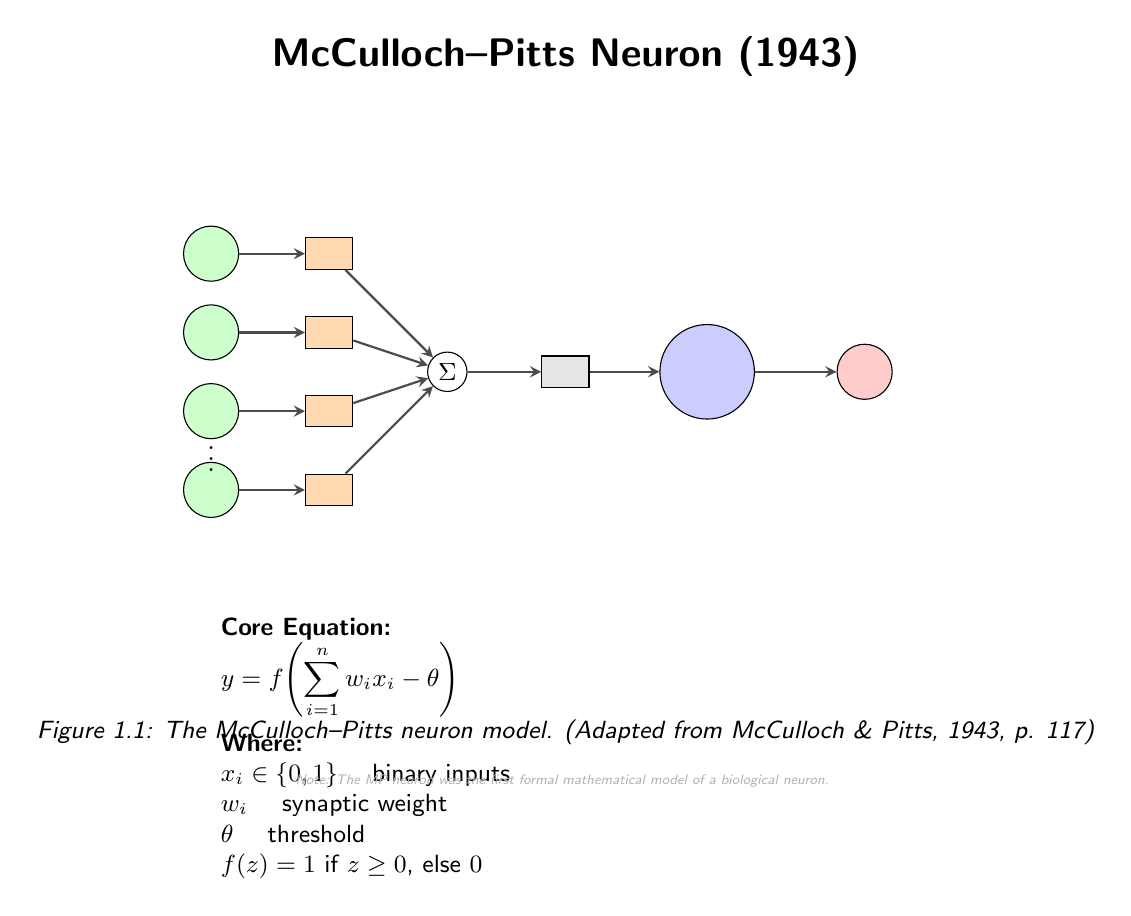
\begin{tikzpicture}[
    % Node styles
    neuron/.style={draw, circle, minimum size=1cm, inner sep=0pt, fill=blue!20},
    input/.style={draw, circle, minimum size=0.7cm, inner sep=0pt, fill=green!20},
    output/.style={draw, circle, minimum size=0.7cm, inner sep=0pt, fill=red!20},
    weight/.style={draw, rectangle, minimum width=0.6cm, minimum height=0.4cm, fill=orange!30, font=\tiny},
    threshold/.style={draw, rectangle, minimum width=0.6cm, minimum height=0.4cm, fill=gray!20, font=\tiny},
    label/.style={font=\sffamily\small},
    title/.style={font=\sffamily\Large\bfseries},
    caption/.style={font=\sffamily\small\itshape},
    edge/.style={-stealth, thick, draw=black!70},
    sum/.style={draw, circle, minimum size=0.5cm, inner sep=0pt, fill=white, font=\sffamily\small},
]

% ============================================================
% Title
% ============================================================
\node[title] at (0, 4.5) {McCulloch–Pitts Neuron (1943)};

% ============================================================
% Inputs
% ============================================================
\node[input, label={[label]below:$x_1$}] (x1) at (-4.5, 2) {};
\node[input, label={[label]below:$x_2$}] (x2) at (-4.5, 1) {};
\node[input, label={[label]below:$x_3$}] (x3) at (-4.5, 0) {};
\node[input, label={[label]below:$x_n$}] (xn) at (-4.5, -1) {};

% Dots
\node at (-4.5, -0.5) {$\vdots$};

% ============================================================
% Weights
% ============================================================
\node[weight, label={[label]above:$w_1$}] (w1) at (-3, 2) {};
\node[weight, label={[label]above:$w_2$}] (w2) at (-3, 1) {};
\node[weight, label={[label]above:$w_3$}] (w3) at (-3, 0) {};
\node[weight, label={[label]above:$w_n$}] (wn) at (-3, -1) {};

% ============================================================
% Summation Node
% ============================================================
\node[sum] (sum) at (-1.5, 0.5) {$\Sigma$};

% ============================================================
% Threshold
% ============================================================
\node[threshold, label={[label]above:$\theta$}] (theta) at (0, 0.5) {};

% ============================================================
% Neuron Body
% ============================================================
\node[neuron, minimum size=1.2cm, label={[label]above:$f$}] (neuron) at (1.8, 0.5) {};

% ============================================================
% Output
% ============================================================
\node[output, label={[label]below:$y \in \{0,1\}$}] (y) at (3.8, 0.5) {};

% ============================================================
% Edges (Input → Weights → Sum → Threshold → Neuron → Output)
% ============================================================
\draw[edge] (x1) -- (w1);
\draw[edge] (x2) -- (w2);
\draw[edge] (x3) -- (w3);
\draw[edge] (xn) -- (wn);

\draw[edge] (w1) -- (sum);
\draw[edge] (w2) -- (sum);
\draw[edge] (w3) -- (sum);
\draw[edge] (wn) -- (sum);

\draw[edge] (sum) -- (theta);
\draw[edge] (theta) -- (neuron);
\draw[edge] (neuron) -- (y);

% ============================================================
% Equations / Legend
% ============================================================
\node[align=left, font=\sffamily\small, anchor=north west] at (-4.5, -2.5) {
  \textbf{Core Equation:} \\
  $\displaystyle y = f\!\left( \sum_{i=1}^{n} w_i x_i - \theta \right)$ \\
  \\
  \textbf{Where:} \\
  $x_i \in \{0,1\}$ \quad binary inputs \\
  $w_i$ \quad synaptic weight \\
  $\theta$ \quad threshold \\
  $f(z) = 1$ if $z \geq 0$, else $0$
};

% ============================================================
% Caption
% ============================================================
\node[caption, anchor=north] at (0, -3.8) {
  Figure 1.1: The McCulloch–Pitts neuron model. (Adapted from McCulloch \& Pitts, 1943, p. 117)
};

% ============================================================
% Historical Note
% ============================================================
\node[align=center, font=\sffamily\tiny, anchor=north, text=gray!60] at (0, -4.5) {
  \textit{Note: The MP neuron was the first formal mathematical model of a biological neuron.}
};

\end{tikzpicture}

\end{document}